\subsection{Pure Observable Objects}
	\label{poo}
	Pure Observable Objects (POO) es el framework que implementa el
	aspecto Observable planteado en la Sección \ref{aspectoObservable}.
	La implementación interna del aspecto agrega un
	atributo llamado \lstinline|changeSupport| del tipo
	\lstinline|PropertySupport| al objeto al que se le aplica el aspecto.
	\lstinline|PropertySupport| es una interfaz, la implementación concreta a
	utilizar se obtiene del el archivo de configuración.
	
	Para completar el objetivo se agregan los métodos 
	\lstinline|addPropertyChangeListener| y
	\lstinline|removePropertyChangeListener| que permiten agregar 
	y remover observadores, y \lstinline|firePropertyChange|
	que notifica a los observadores que un atributo ha cambiado.
	
	Para entender mejor el modelo de classes, la la figura \ref{fig:poo} muesta
	esquemáticamente el diseño de la herramienta.
	
	\begin{figure}
		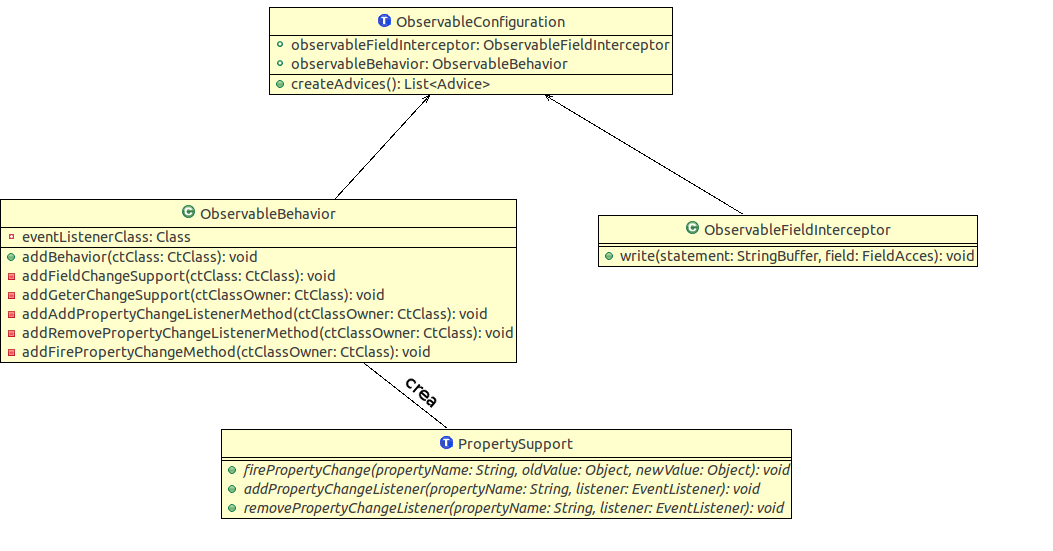
\includegraphics[width=450px, height=200px]{img/poo}
	 	\label{fig:poo}
	 	\caption{}
	\end{figure}
	
	Para agregarle este aspecto a una clase se utiliza la \emph{Annotation}
	\lstinline|Observable|.
	
	\begin{lstlisting} 
		@Observable
		public class Client{
		}
	\end{lstlisting}
